\subsection{Describe the He spectrum (singlet and triplet states) and explain why it was initially believed that there are two kinds of helium (called para- and orthohelium).}


\begin{figure}[!h]
    \centering
    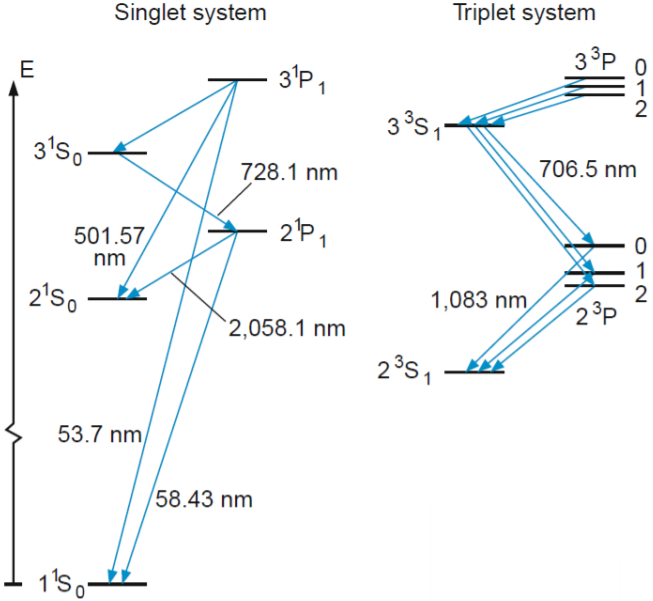
\includegraphics[width=0.7\textwidth]{Q12/images/SingletOgtripletTilstandeIHelium.PNG}
    \caption{De tilladte overgange mellem niveauer i helium styres af udvagsreglerne $\Delta S = 0$, som undgår overgange mellem singlet- og tripletsystemet, og $\Delta L = \pm 1$. Siden at der ikke er overgange mellem singlet- og tripletsystemet er det smart at tegne disse hver for sig, og det blev tidligere troet, at disse var to forskellige typer af helium, som blev kaldt hhv. parahelium og ortohelium.}
    \label{fig:Q12_SingletOgTripletTilstandeIHelium}
\end{figure}

\Cref{fig:Q12_SingletOgTripletTilstandeIHelium} kan vi se heliums spektrum. Det bemærkes, at vi kun har overgange indbyrdes i de to ''dele'' af hydrogen, hvilket skyldes udvalgsreglen for $\Delta s$:

Det totale spinkvantetal ændres ikke ved overgange grundet den elektriske dipolapproksimation. I matrixelementet vil man få
\begin{align}
    \bra{\Psi_\text{final}}r\ket{\Psi_\text{initial}} \: ,
\end{align}
men operatoren $r$ virker ikke på spinet, hvorfor man vil få (''final'' skrives f og ''initial'' i)
\begin{align}
    \braket{\chi_f}{\chi_i}\bra{\psi_f}r\ket{\psi_i} \propto \delta_{f,i} \: ,
\end{align}
altså matrixelementet vil give 0, medmindre $\Delta s = 0$.

Af denne grund blev det førhen troet, at der var tale om to typer af helium: \textsf{parahelium} og \textsf{ortohelium}, som er henholdsvis singlettilstanden og triplettilstanden.


\paragraph{Symmetriske og antisymmetriske rummelige bølgefunktioner:} Vi betragter to elektroner i hhv. tilstanden 1s (altså $n=1$ og $l=0$) og en vilkårlig tilstand $n,\,l$. Med en stadig negligeret interaktion mellem de to elektroner ser vi stadig bølgefunktionen som værende et produkt af bølgefunktionen for hver af elektronerne, $\psi = \psi(1)\psi(2)$, hvorfor
\begin{align}
    \psi_\text{sp}(1,2) &= \psi_{1s}(1)\psi_{nl}(2) \: , \quad \text{og} \\
    \psi_\text{sp}(2,1) &= \psi_{1s}(2)\psi_{nl}(1) \: ,
\end{align}
da vi har tale om identiske partikler. Disse er enrgimæssigt udartede (eng. energetically degenerate), men i stdet for at gå i gang med udartet perturbationsteori kan man tænkte smart og undgå perturbationsteori ved at gøre brug af de rigtige argumenter.

Idet at vi har tale om identiske partikler må det gøre sig gældende, at
\begin{align}
    \abs{\psi_\text{sp}(1,2)}^2 &= \abs{\psi_\text{sp}(2,1)}^2 \: ,
\end{align}
og benytter vi \textsf{permutationsoperatoren} (eng. exchange operator) $P$, hvorom det gælder, at
\begin{align}
    P^2 \psi(1,2) &= \psi(1,2) \: , \quad \text{og} \label{eq:Q12_ExchangeOperatorDefinitions1} \\
    P \psi(1,2) &= \psi(2,1) \: ,\label{eq:Q12_ExchangeOperatorDefinitions2}
\end{align}
og som har egenvektorfunktionerne
\begin{align}
    P^2 \psi &= p^2 \psi \: , \quad \text{og} \label{eq:Q12_ExchangeOperatorEingenValueFunctions1} \\
    P \psi &= p \psi \: , \label{eq:Q12_ExchangeOperatorEingenValueFunctions2}
\end{align}
da får vi, at
\begin{align}
    \abs{\psi_\text{sp}(1,2)}^2 &= \abs{\psi_\text{sp}(2,1)}^2
    = \abs{P\psi_\text{sp}(1,2)}^2
    = \abs{p\psi_\text{sp}(1,2)}^2
    = \abs{p}^2 \abs{\psi_\text{sp}(1,2)}^2 \nonumber\\
    \Rightarrow \abs{p}^2 &= 1 \: .
\end{align}
Dette betyder, at brugen af permutationsoperatoren ikke kan ændre amplituden af bølgefunktionen, som den benyttes på, hvorfor den må ændre fasen i stedet, hvilken er givet ved
\begin{align} \label{eq:Q12_FaseskiftP}
    p &= \exp{i\phi} \: ,
\end{align}
hvor $\phi$ er vinklen for faseskiftet.

Sammenligner vi nu \cref{eq:Q12_ExchangeOperatorDefinitions1} med \cref{eq:Q12_ExchangeOperatorEingenValueFunctions1} kan det ses, at
\begin{align}
    \psi(1,2) &= P^2 \psi(1,2) = p^2 \psi(1,2) \nonumber\\
    \Rightarrow p^2 = 1 \: .
\end{align}
Benytter vi nu dette med \cref{eq:Q12_FaseskiftP}, så fås
\begin{align}
    1 &= p^2 = \left(\exp{i\phi}\right)^2 = \exp{2i\phi} \nonumber\\
    \Rightarrow \phi &= k\pi \: , \quad \forall k \in \mathbb{N}_0 \: .
\end{align}
Dette indsættes nu i \cref{eq:Q12_FaseskiftP}, hvorved vi kan finde $p$
\begin{align}
    p &= \exp{i\phi} =
        \begin{cases}
            \exp(i \cdot 0) = \exp(0) = 1 \\
            \exp(i\pi) = \cos(\pi) + i\sin(\pi) = \cos(\pi) = -1
        \end{cases} \: ,
\end{align}
altså $p = \pm 1$.

Ved at benytte, at $p = \pm 1$, så kan det ses, at
\begin{align} \label{eq:Q12_SymmetrikravTilBoelgefunktionerne}
    \psi(1,2) &= P\psi(2,1) = p\psi(2,1) = \pm \psi(2,1) \: .
\end{align}
Vi kan altså have bølgefunktioner, som er symmetriske ($+$) eller antisymmetriske ($-$) under ombytning. For at opfylde symmetrikravene i \cref{eq:Q12_SymmetrikravTilBoelgefunktionerne} dannes to bølgefunktioner for de to elektroner
\begin{align}
    \psi^S(1,2) &= \frac{1}{\sqrt{2}} \left\{\psi_{1s}(1)\psi_{nl}(2) + \psi_{1s}(2)\psi_{nl}(1)\right\} \: , \quad \text{og} \\
    \psi^S(1,2) &= \frac{1}{\sqrt{2}} \left\{\psi_{1s}(1)\psi_{nl}(2) - \psi_{1s}(2)\psi_{nl}(1)\right\} \: ,
\end{align}
hvor $S$ og $A$ angiver om der er tale om den hhv. symmetriske eller antisymmetriske bølgefunktion.


\paragraph{Symmetriske og antisymmetriske spinbølgefunktioner:} Ovenfor har vi behandlet de rummelige bølgefunktioner, men vi ved, at elektronen har et spin, som også skal medtages i den totale bølgefunktion, $\Psi = \psi(\Vec{r}) \otimes \chi(\Vec{s})$, for at denne beskriver systemet. De mulige spinbølgefunktioner for to spin-$1/2$ partikler er
\begin{align}
    \ket{\uparrow\uparrow} \: , \quad \ket{\uparrow\downarrow} \: , \quad \ket{\downarrow\uparrow} \: , \quad \text{og} \quad \ket{\downarrow\downarrow} \: .
\end{align}
Disse skal være egenfunktioner for $\Vec{s}^2$, hvilket kun gør sig gældende for $\ket{\uparrow\uparrow}$ og $\ket{\downarrow\downarrow}$, hvorfor de to andre ''redefineres'', således at vi får de følgende symmetriske og antisymmetriske spinbølgefunktioner
\begin{align}
    \chi^S &= \ket{\uparrow\uparrow} \: , \qquad \qquad \qquad \quad \text{hvor} \quad m_s = 1 \: , \\
    \chi^S &= \ket{\downarrow\downarrow} \: , \qquad \qquad \qquad \quad \text{hvor} \quad m_s = -1 \: , \\
    \chi^S &= \frac{1}{\sqrt{2}} \Big(\ket{\uparrow\downarrow} + \ket{\downarrow\uparrow}\Big) \: , \,\quad \text{hvor} \quad m_s = 0 \: , \\
    \chi^A &= \frac{1}{\sqrt{2}} \Big(\ket{\uparrow\downarrow} - \ket{\downarrow\uparrow}\Big) \: , \,\quad \text{hvor} \quad m_s = 0 \: .
\end{align}
Triplettilstanden (de symmetriske spinbølgefunktioner) har altså $s = 1$, mens singlettilstanden (den antisymmetriske spinbølgefunktion) har $s = 0$.


\paragraph{Mulige bølgefunktioner respekterende Paulis udelukkelsesprincip:} Paulis udelukkelseprincip siger i sin korthed, at den totale bølgefunktion for et system med mere end én identisk fermion altid skal være antisymmetrisk under ombytning af disse fermioner. Det vil sige, at de mulige totalbølgefunktioner vil være
\begin{align}
    \Psi &= \psi^S \otimes \chi^A \: , \quad \text{og} \\
    \Psi &= \psi^A \otimes \chi^S \: ,
\end{align}
hvor den første bølgefunktion vil give en singlettilstand, da $S = 0$, hvormed multipliciten\footnote{Se termsymbol i disposition 14.} er $2S + 1 = 1$, og den anden mulighed giver en triplettilstand, da $S = 1$, hvormed multipliciteten er $2S + 1 = 3$.

Kigger vi på grundtilstanden i helium er der kun én mulig bølgefunktion
\begin{align}
    \Psi &= \psi^S \otimes \chi^A = \frac{1}{2} \Big\{\psi_{1s}(1)\psi_{nl}(2) + \psi_{1s}(2)\psi_{nl}(1)\Big\}\Big(\ket{\uparrow\downarrow} - \ket{\downarrow\uparrow}\Big) \: ,
\end{align}
idet at en antisymmetrisk bølgefunktion ville give $0$, da $\psi_{1s}(1)\psi_{1s}(2) =\psi_{1s}(2)\psi_{1s}(1)$.

Kigger vi nu i stedet på helium med én exciteret elektron, således at $n_1 = 2$, mens $n_2 = 1$ og $l_2 = 0$, så vil de følgende tilstande være mulige
\begin{align}
    2^1S_0 &\quad \left(l_1 = 0,\: m_{l_1} = 0, \: m_{s_1} = -\frac{1}{2}, \: J = 0\right) \: , \\
    2^1P_1 &\quad \left(l_1 = 1,\: m_{l_1} = 0,\pm1, \: m_{s_1} = -\frac{1}{2}, \: J = 1\right) \: , \\
    2^3S_1 &\quad \left(l_1 = 0,\: m_{l_1} = 0, \: m_{s_1} = \frac{1}{2}, \: J = 1\right) \: , \\
    2^3P_0 &\quad \left(l_1 = 1,\: m_{l_1} = -1, \: m_{s_1} = \frac{1}{2}, \: J = 0\right) \: , \\
    2^3P_1 &\quad \left(l_1 = 1,\: m_{l_1} = 0, \: m_{s_1} = \frac{1}{2}, \: J = 1\right) \: , \\
    2^3P_2 &\quad \left(l_1 = 1,\: m_{l_1} = 1, \: m_{s_1} = \frac{1}{2}, \: J = 2\right) \: ,
\end{align}
hvilke kan ses af \cref{fig:Q12_SingletOgTripletTilstandeIHelium}.

På \cref{fig:Q12_SingletOgTripletTilstandeIHelium} kan der bemærkes lidt forskelligt:
\begin{itemize}
    \item Der findes ikke et $(1s)(1s)$ grundtilstand i triplettilstnden, da dette ville give $\psi^S = 0$.
    \item For $L = 0$ (S-obitaltilstande) forekommer der ikke nogen energiopsplitning til ''triplettilstande''.
    \item For $L \ne 0$ kommer opsplitningerne af finstrukturen, som opsplitter mht. $J$.
    \item Der findes ingen overgange mellem singlet- og tripletsystemerne, da udvalgsreglen omkring $\Delta S = 0$ forbyder at gå mellem $S = 0$ og $S = 1$ tilstandene.
    \begin{itemize}
        \item Tidligere blev det troet, at de to systemer var to forskellige typer af helium (da disse to systemer aldrig skiftede mellem hinanden), hvor singletsystemet blev kaldt \textsf{parahelium}, og tripletsystemet blev kaldt \textsf{ortohelium}.
    \end{itemize}
\end{itemize}